\documentclass{article}
\begin{document}

The techniques of motions captures presented in section \ref{sec:motionCaptureTech} have the disadvantage to be expensive and difficult to use. The 3D motion camera tracking system using marker is even criticized as been unreliable for hand motion tracking. In order to propose a data collection benchmark that is reliable and easily reproducible, we present the use of a different device that is able to perform hand tracking quickly and for a reasonable amount of money.

The Oculus Quest is a virtual reality headset developed by Facebook (\url{https://www.oculus.com/quest/}). It has 4 infra-red mounted cameras which are oriented to film the user hands from different angles. The headset is then able to reconstruct in real time a pair of 3D hands which accurately match the user gestures. The pose reconstruction technique is similar different from a conventional motion tracking system as it does not need any marker on the subject. It relies on a deep neural network which only takes to camera vision as input and uses an architechture similar to PoseNets; a model from TensorFlow used for human posture estimation (\url{https://www.tensorflow.org/lite/examples/pose_estimation/overview}) \cite{ref:oculus1, ref:oculus2}.

\subsubsection{Advantages of the Oculus Quest device}
\begin{itemize}
	\item It is cheap compared to the others (399 euros)
	\item It can estimate 26 degrees of freedom for each hand \cite{ref:oculus2}
	\item The neural network is specifically trained to estimate hand gesture which allows more accurate estimation than conventional motion tracking
	\url{https://developer.oculus.com/documentation/unity/unity-utilities-overview/})
	\item It is fast to setup for data collection
	\item It can be controlled remotely using a USB-c cable
	\item A programming library is available to easily use it (OVR library for the Unity game engine
	\item The programming library provides additional pieces of information like the quality of the estimation for each finger and a pinching boolean that tells if a given finger is touching the thumb of the same hand.
\end{itemize}

\subsubsection{Disadvantages of the Oculus Quest device}
\begin{itemize}
	\item The precision of the estimation is not the same for all fingers
	\item If a single joint is incorrectly predicted, it can cause big prediction errors \cite{ref:oculus1}
	\item If the background color is similar to the skin color, the estimation becomes less accurate \cite{ref:oculus1}
	\item There is no documentation on the accuracy of the estimation. We can only rely on testers feeling about it \cite{ref:oculus3}
	\item Its sampling rate is quite low (50 or 60Hz depending on the electrical frequency in the country)
\end{itemize}


\subsubsection{Unity}

In order to collect the data of the gesture estimation from the Oculus Quest, we need to use the Unity game engine (\url{https://unity.com/}). It is a really easy to use framework that enables to build 3D scenes and can be programmed in $C\#$. It has a lot of documentation, receives regular update since 2005 and has a huge community of developers. There also exist an asset store which enables to download lots of assets to put in the built software.\cite{ref:oculus4}

\paragraph{The OVR library}

To use the Oculus quest components from a Unity project, we need to use the Unity OVR library (\url{https://developer.oculus.com/documentation/unity/unity-utilities-overview/}) which provides all the classes that allows to use the hand tracking option of the headset and to collect its data. When it is setup, the user is able to see its hands in the virtual reality and to program can get, at each frame (50 frames per seconds), the rotation of each bone of the 2 hands as well as the additional information provided by the library.

\begin{figure}[h]
	\centering
	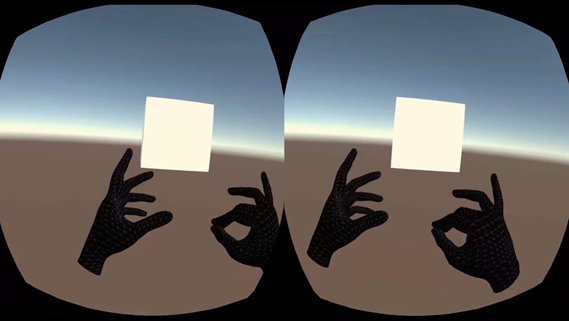
\includegraphics[width=10cm]{images/questView.png}
	\caption{View of the estimated hands from the Oculus quest Virtual Reality headset}
	\label{fig:cyberGlove3}
\end{figure}

The information that can be collected for each hand and at each frame from the headset is:
\begin{enumerate}
	\item The position and rotation of the hand in the 3D space
	\item The 3D rotation of 17 bones of the hand
	\item A boolean telling if the estimation could be processed (false means that the neural network failed to predict the pose)
	\item A boolean per finger indicating if the quality of the estimation of its pose is high or low
	\item A boolean per finger, except the thumb, indicating if it is touching the thumb of the same hand (pinching)
\end{enumerate}
The device is also able to compute the UTC timestamps of each frame which can b used for synchronization.

\paragraph{The Hand Tracking Gesture Recorder library}

The OVR library can be completed with a hand gesture data collection library (\url{https://github.com/jorgejgnz/HandTrackingGestureRecorder}). Made by Jorge Juan González (HCI Researcher at I3A (UCLM)), it enables to record a pose of the hand using the Oculus Quest so that that, later, the program produces a trigger when the user does the same pose. It is possible to save multiple gestures in a file and load them when starting the program on the headset.

This library takes as input all the bones of the hand and tries, based on their relative position to the wrist, to find the pose, among the recorded ones, that is the more probable to be the current pose. If no pose has a high enough probability, it does not output any prediction.

\end{document}